\section{熵正则化}
\label{sec:ot-entropic}

$m$个源点、$n$个目标点的运输线性规划有$mn$个变量。分布由细网格离散化时，$m,n$成千上万，单纯形类方法要在巨大的多面体顶点之间移动，而且最优解落在边界上，对数据的微小变化不连续。一个常用的办法是在成本上加一个惩罚，鼓励方案“散开”一些：散开的方案位于多面体内部，最优性条件变成光滑的方程，可以用简单的交替缩放求解。代价是求得的不再是原问题的最优方案。本节研究这一权衡。

\paragraph{正则化问题}
设$\bm{a}\in\mathbb{R}^{m}$，$\bm{b}\in\mathbb{R}^{n}$是概率向量。若某个$a_i=0$，任何可行方案的第$i$行都必须为零，这一行可以直接删去；对$b_j=0$的列也一样。所以下面总设$\bm{a},\bm{b}$的各分量都为正。以边缘乘积$\bm{a}\otimes\bm{b}$，即独立方案$(a_ib_j)_{i,j}$为参考，对$\varepsilon>0$考虑
\begin{equation}
 \min_{\bm{\pi}\in U(\bm{a},\bm{b})}\ L_\varepsilon(\bm{\pi}),\qquad L_\varepsilon(\bm{\pi})=\langle\bm{C},\bm{\pi}\rangle+\varepsilon D_{\mathrm{KL}}(\bm{\pi}\Vert\bm{a}\otimes\bm{b}),
 \label{eq:ot-entropic-problem}
\end{equation}
其中
\[
 D_{\mathrm{KL}}(\bm{\pi}\Vert\bm{a}\otimes\bm{b})=\sum_{i,j}\pi_{i,j}\ln\frac{\pi_{i,j}}{a_ib_j},
\]
约定$0\ln0=0$。这一问题称为\term{熵正则化最优运输}（entropic optimal transport）。

两项各有含义。$\langle\bm{C},\bm{\pi}\rangle$是原来的运输成本；KL项是方案偏离独立方案的程度。把$\bm{\pi}$看成$(X,Y)$的联合分布，它的两个边缘是$\bm{a},\bm{b}$，所以这一项正是第~\ref{chap:information-measures}章的互信息$I(X;Y)$：它衡量知道源位置后，对目标位置的不确定性减少了多少。$\varepsilon$很大时，惩罚迫使方案接近独立方案，源与目标几乎无关；$\varepsilon\to0$时，方案回到原问题的最优方案，源几乎决定目标。图~\ref{fig:ot-entropic-plans}在一个细网格上展示这一变化。

\begin{BookInlineFigure}
 \centering
 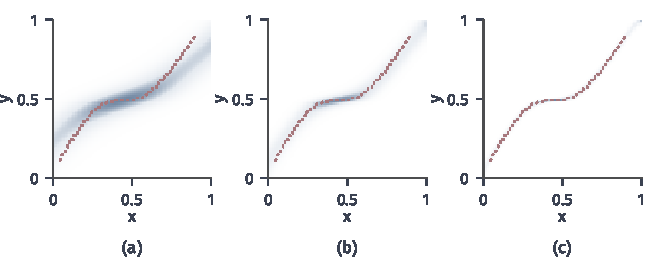
\includegraphics[width=112mm]{figures/07-probability/07-distribution-optimization/matplotlib/ot-entropic-plans/figure.pdf}
 \caption{$[0,1]$上$80$个格点的熵正则化方案，源为双峰分布，目标为单峰分布，平方成本。图中是按行归一化后的方案，即给定$x$时$y$的条件分布，颜色越深概率越大；红色点线是不加正则化时的单调最优映射。(a)$\varepsilon=0.02$。(b)$\varepsilon=0.005$。(c)$\varepsilon=0.0005$。}
 \label{fig:ot-entropic-plans}
\end{BookInlineFigure}

\paragraph{对偶问题与原对偶差}
正则化问题的对偶变量仍是一对向量$\bm{f}\in\mathbb{R}^{m}$，$\bm{g}\in\mathbb{R}^{n}$，但约束$f_i+g_j\leq c_{i,j}$换成一个光滑的惩罚：
\begin{equation}
 D_\varepsilon(\bm{f},\bm{g})=\langle\bm{a},\bm{f}\rangle+\langle\bm{b},\bm{g}\rangle-\varepsilon\sum_{i,j}a_ib_j\Bigl(\mathrm{e}^{(f_i+g_j-c_{i,j})/\varepsilon}-1\Bigr).
 \label{eq:ot-entropic-dual}
\end{equation}
违反约束越多，指数项越大；$\varepsilon\to0$时，它趋于“满足约束为$0$、违反约束为$-\infty$”的硬约束。下面的引理是第~\ref{sec:ot-potentials}节式~\eqref{eq:ot-gap}的对应物。

\begin{lemma}[正则化问题的原对偶差]
\label{lem:ot-entropic-gap}
对$\bm{\pi}\in U(\bm{a},\bm{b})$与任意$\bm{f},\bm{g}$，记$r_{i,j}=\pi_{i,j}/(a_ib_j)$，$s_{i,j}=(f_i+g_j-c_{i,j})/\varepsilon$。则
\begin{equation}
 L_\varepsilon(\bm{\pi})-D_\varepsilon(\bm{f},\bm{g})=\varepsilon\sum_{i,j}a_ib_j\bigl(r_{i,j}\ln r_{i,j}-r_{i,j}-r_{i,j}s_{i,j}+\mathrm{e}^{s_{i,j}}\bigr)\geq0 ,
 \label{eq:ot-entropic-gap}
\end{equation}
每一项取等当且仅当$r_{i,j}=\mathrm{e}^{s_{i,j}}$。
\end{lemma}

\begin{proof}
由行列约束，
\[
 \langle\bm{a},\bm{f}\rangle+\langle\bm{b},\bm{g}\rangle=\sum_{i,j}\pi_{i,j}(f_i+g_j);
\]
又$\bm{a}\otimes\bm{b}$与$\bm{\pi}$的元素总和都是$1$。代入式~\eqref{eq:ot-entropic-dual}，
\[
 L_\varepsilon(\bm{\pi})-D_\varepsilon(\bm{f},\bm{g})=\sum_{i,j}\pi_{i,j}(c_{i,j}-f_i-g_j)+\varepsilon\sum_{i,j}\pi_{i,j}\ln r_{i,j}+\varepsilon\sum_{i,j}a_ib_j\mathrm{e}^{s_{i,j}}-\varepsilon .
\]
把$\pi_{i,j}(c_{i,j}-f_i-g_j)$写成$-\varepsilon a_ib_jr_{i,j}s_{i,j}$，把常数$\varepsilon$写成$\varepsilon\sum_{i,j}a_ib_jr_{i,j}$，即得等式。

对固定的$r\geq0$，函数$s\mapsto\mathrm{e}^{s}-rs$在$r>0$时于$s=\ln r$处取最小值$r-r\ln r$，所以
\[
 r\ln r-r-rs+\mathrm{e}^{s}\geq r\ln r-r+r-r\ln r=0 ,
\]
等号当且仅当$s=\ln r$；$r=0$时这一项是$\mathrm{e}^{s}>0$。
\end{proof}

\begin{theorem}[熵正则化问题的解]
\label{thm:ot-entropic-solution}
设$\bm{a},\bm{b}$各分量为正，$\bm{C}$各元素有限，$\varepsilon>0$。则问题~\eqref{eq:ot-entropic-problem}有唯一解$\bm{\pi}^{\varepsilon}$，它的各元素都为正，并且存在$\bm{f},\bm{g}$使
\begin{equation}
 \pi^{\varepsilon}_{i,j}=a_ib_j\,\mathrm{e}^{(f_i+g_j-c_{i,j})/\varepsilon}.
 \label{eq:ot-entropic-form}
\end{equation}
这样的$(\bm{f},\bm{g})$使$D_\varepsilon$取最大值，并且最大值等于$L_\varepsilon(\bm{\pi}^{\varepsilon})$。反过来，$U(\bm{a},\bm{b})$中任何形如式~\eqref{eq:ot-entropic-form}的方案都是唯一解。
\end{theorem}

\begin{proof}
\emph{存在与唯一。}$t\mapsto t\ln t$在$[0,\infty)$上连续，所以$L_\varepsilon$在紧集$U(\bm{a},\bm{b})$上连续，最小值取得。$t\mapsto t\ln(t/(a_ib_j))$严格凸，成本项是线性的，所以$L_\varepsilon$在凸集$U(\bm{a},\bm{b})$上严格凸，最小点唯一。

\emph{各元素为正。}设可行的$\bm{\pi}$有零元素。对$0<\lambda<1$令
\[
 \bm{\pi}^{\lambda}=(1-\lambda)\bm{\pi}+\lambda\,\bm{a}\otimes\bm{b},
\]
它是两个可行方案的凸组合，仍可行。成本项与$\bm{\pi}$的正元素对应的熵项都是$\lambda$的可微函数，它们的变化不超过$K\lambda$（$K$为常数，$\lambda$足够小）。$\bm{\pi}$的零元素$(i,j)$处，熵项从$0$变为
\[
 \lambda a_ib_j\ln\frac{\lambda a_ib_j}{a_ib_j}=\lambda a_ib_j\ln\lambda .
\]
记$\kappa>0$为零元素处$a_ib_j$之和，则
\[
 L_\varepsilon(\bm{\pi}^{\lambda})-L_\varepsilon(\bm{\pi})\leq\lambda\bigl(K+\varepsilon\kappa\ln\lambda\bigr),
\]
$\lambda$足够小时右边为负。所以有零元素的方案不是最小点。

\emph{缩放形式。}最小点$\bm{\pi}^{\varepsilon}$各元素为正，对任何行和、列和都为零的矩阵$\bm{D}$，$\bm{\pi}^{\varepsilon}+t\bm{D}$在$\lvert t\rvert$很小时可行。$t\mapsto L_\varepsilon(\bm{\pi}^{\varepsilon}+t\bm{D})$在$t=0$处取最小，导数为零：
\[
 \sum_{i,j}D_{i,j}h_{i,j}=0,\qquad h_{i,j}=c_{i,j}+\varepsilon\ln\frac{\pi^{\varepsilon}_{i,j}}{a_ib_j}+\varepsilon .
\]
对$i<m$，$j<n$取$\bm{D}$在$(i,j),(m,n)$处为$1$、在$(i,n),(m,j)$处为$-1$、其余为$0$，它的行和、列和都是零，代入得
\[
 h_{i,j}=(h_{i,n}-h_{m,n})+h_{m,j} .
\]
令$\alpha_i=h_{i,n}-h_{m,n}$，$\beta_j=h_{m,j}$，可以逐一核对$h_{i,j}=\alpha_i+\beta_j$对包括末行末列在内的一切$i,j$成立。取$f_i=\alpha_i-\varepsilon$，$g_j=\beta_j$，解出$\pi^{\varepsilon}_{i,j}$即得式~\eqref{eq:ot-entropic-form}。

\emph{对偶。}式~\eqref{eq:ot-entropic-form}说的就是$r_{i,j}=\mathrm{e}^{s_{i,j}}$，由引理~\ref{lem:ot-entropic-gap}，原对偶差为零。对任何$(\bm{f}',\bm{g}')$，同一引理说明它的对偶值不超过$L_\varepsilon(\bm{\pi}^{\varepsilon})$，而$(\bm{f},\bm{g})$的对偶值等于它，所以$(\bm{f},\bm{g})$使$D_\varepsilon$最大。反过来，可行且形如式~\eqref{eq:ot-entropic-form}的方案使原对偶差为零，它的$L_\varepsilon$值等于一个下界，是最小点。
\end{proof}

记$u_i=\mathrm{e}^{f_i/\varepsilon}$，$v_j=\mathrm{e}^{g_j/\varepsilon}$，以及正矩阵
\begin{equation}
 K_{i,j}=a_ib_j\,\mathrm{e}^{-c_{i,j}/\varepsilon},
 \label{eq:ot-gibbs-kernel}
\end{equation}
式~\eqref{eq:ot-entropic-form}写成
\begin{equation}
 \bm{\pi}^{\varepsilon}=\operatorname{diag}(\bm{u})\,\bm{K}\operatorname{diag}(\bm{v}).
 \label{eq:ot-scaling-form}
\end{equation}正则化解是固定矩阵$\bm{K}$的行与列分别乘上一个正因子。问题于是变成：找正向量$\bm{u},\bm{v}$，使缩放后的矩阵行和为$\bm{a}$、列和为$\bm{b}$。

\paragraph{正则化目标与运输成本}
正则化问题的解给出两个数：正则化目标值$L_\varepsilon(\bm{\pi}^{\varepsilon})$，以及它的运输成本$\langle\bm{C},\bm{\pi}^{\varepsilon}\rangle$。两者都不等于原问题的最优值$\operatorname{OT}$，必须分开记录。设$\bm{\pi}^{*}$是原问题的一个最优方案。$\bm{\pi}^{\varepsilon}$使$L_\varepsilon$最小，所以它的$L_\varepsilon$值不超过$\bm{\pi}^{*}$的值；再利用KL非负，
\begin{equation}
 0\leq\langle\bm{C},\bm{\pi}^{\varepsilon}\rangle-\operatorname{OT}\leq\varepsilon D_{\mathrm{KL}}(\bm{\pi}^{*}\Vert\bm{a}\otimes\bm{b})\leq\varepsilon\min\bigl(H(\bm{a}),H(\bm{b})\bigr),
 \label{eq:ot-entropic-bias}
\end{equation}
熵以奈特计。左边的不等式是因为$\bm{\pi}^{\varepsilon}$可行；最后一步是因为互信息不超过任一边缘的熵（第~\ref{chap:information-measures}章）。所以运输成本的偏差随$\varepsilon$线性地趋于零。

全章例子中，$\bm{\pi}^{*}$是逐格搬运，
\[
 \begin{aligned}
 D_{\mathrm{KL}}(\bm{\pi}^{*}\Vert\bm{a}\otimes\bm{b})&=2\times0.2\ln\frac{0.2}{0.1}+2\times0.3\ln\frac{0.3}{0.15}\\
 &=\ln2\approx0.693 .
 \end{aligned}
\]
$\varepsilon=1$时数值求得$\langle\bm{C},\bm{\pi}^{\varepsilon}\rangle\approx0.814$，偏差$0.214$，在上界$0.693$之内；正则化目标值约为$1.087$，比运输成本还多出$\varepsilon D_{\mathrm{KL}}(\bm{\pi}^{\varepsilon}\Vert\bm{a}\otimes\bm{b})\approx0.272$。图~\ref{fig:ot-entropic-bias}画出两者随$\varepsilon$的变化：$\varepsilon\to\infty$时运输成本趋于独立方案的$1.58$，$\varepsilon\to0$时趋于$0.6$。

\begin{BookInlineFigure}
 \centering
 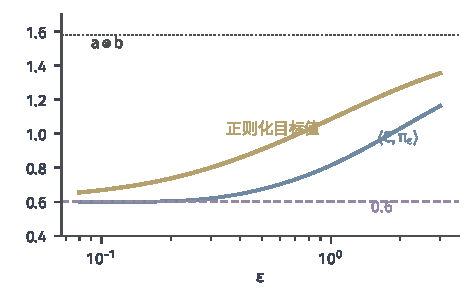
\includegraphics[width=80mm]{figures/07-probability/07-distribution-optimization/matplotlib/ot-entropic-bias/figure.pdf}
 \caption{全章例子的熵正则化偏差，横轴为$\varepsilon$（对数刻度）。蓝线是正则化解的运输成本$\langle\bm{C},\bm{\pi}^{\varepsilon}\rangle$，黄线是正则化目标值$L_\varepsilon(\bm{\pi}^{\varepsilon})$，紫色虚线是原问题最优值$0.6$，深灰点线是独立方案的成本$1.58$。}
 \label{fig:ot-entropic-bias}
\end{BookInlineFigure}

\subsection{Sinkhorn迭代}
\label{sec:ot-sinkhorn}

要找的是两个缩放向量。若列因子$\bm{v}$已知，行条件$\sum_ju_iK_{i,j}v_j=a_i$对每个$i$只含一个未知数$u_i$，立即解出；反过来，行因子已知时列因子也立即解出。于是交替地做这两件事。

\paragraph{交替缩放}
固定$\bm{v}$，令行和等于$\bm{a}$；再固定新的$\bm{u}$，令列和等于$\bm{b}$：
\begin{equation}
 u_i\leftarrow\frac{a_i}{(\bm{K}\bm{v})_i},\qquad v_j\leftarrow\frac{b_j}{(\bm{K}^{\top}\bm{u})_j}.
 \label{eq:ot-sinkhorn}
\end{equation}
这一迭代称为\term{Sinkhorn迭代}（Sinkhorn iteration）。每半步只满足一组约束，并破坏另一组；交替进行时，两组约束的残差逐步减小。

每半步还有一个优化含义。对式~\eqref{eq:ot-entropic-dual}关于$f_i$求偏导，
\[
 \frac{\partial D_\varepsilon}{\partial f_i}=a_i-\sum_ja_ib_j\mathrm{e}^{(f_i+g_j-c_{i,j})/\varepsilon}=a_i-\sum_ju_iK_{i,j}v_j .
\]
令它为零，就是式~\eqref{eq:ot-sinkhorn}的行更新。$D_\varepsilon$关于$\bm{f}$是凹函数，所以行更新在$\bm{g}$固定时把$D_\varepsilon$对$\bm{f}$精确地最大化，列更新同理。Sinkhorn迭代是对偶问题的交替坐标上升，对偶值逐步增大。

\paragraph{对数域计算}
$\varepsilon$很小时$\mathrm{e}^{-c_{i,j}/\varepsilon}$会下溢为零，$u_i,v_j$则会上溢。改用$\bm{f}=\varepsilon\ln\bm{u}$，$\bm{g}=\varepsilon\ln\bm{v}$表示，行更新中的$a_i$与$K_{i,j}$里的$a_i$相消，得到
\begin{equation}
 f_i\leftarrow-\varepsilon\ln\sum_jb_j\,\mathrm{e}^{(g_j-c_{i,j})/\varepsilon},\qquad g_j\leftarrow-\varepsilon\ln\sum_ia_i\,\mathrm{e}^{(f_i-c_{i,j})/\varepsilon}.
 \label{eq:ot-sinkhorn-log}
\end{equation}
计算$\ln\sum_j\exp(z_j)$时先减去$\max_jz_j$再求指数，结果再加回，所有指数都不超过$1$，不会溢出。式~\eqref{eq:ot-sinkhorn-log}是$c$变换~\eqref{eq:ot-c-transform}的光滑版本：$\varepsilon\to0$时，$-\varepsilon\ln\sum_jb_j\mathrm{e}^{(g_j-c_{i,j})/\varepsilon}$趋于$\min_j(c_{i,j}-g_j)$。

\paragraph{停止判据}
每轮做完列更新后，列和精确等于$\bm{b}$，行和与$\bm{a}$的差$\rho=\lVert\bm{\pi}\bm{1}-\bm{a}\rVert_1$衡量可行性。但当前方案不可行，它的目标值不能直接与最优值比较。为此先把它修成一个可行方案$\tilde{\bm{\pi}}$：行和超过$a_i$的行按比例缩小到$a_i$；列和超过$b_j$的列同样缩小；此时行缺额$\bm{e}_r=\bm{a}-\tilde{\bm{\pi}}\bm{1}$与列缺额$\bm{e}_c=\bm{b}-\tilde{\bm{\pi}}^{\top}\bm{1}$都非负且总和相等，再加上$\bm{e}_r\bm{e}_c^{\top}/\lVert\bm{e}_r\rVert_1$补足。由引理~\ref{lem:ot-entropic-gap}与定理~\ref{thm:ot-entropic-solution}，
\begin{equation}
 0\leq L_\varepsilon(\tilde{\bm{\pi}})-L_\varepsilon(\bm{\pi}^{\varepsilon})\leq L_\varepsilon(\tilde{\bm{\pi}})-D_\varepsilon(\bm{f},\bm{g}),
 \label{eq:ot-sinkhorn-stop}
\end{equation}
右边可以直接算出。它小于容差$\tau$时停止，输出$\tilde{\bm{\pi}}$，并且知道它与正则化最优值的差不超过$\tau$。

\needspace{6\baselineskip}
\paragraph{变量}
\begin{itemize}
 \item $\bm{K}\in\mathbb{R}^{m\times n}$：式~\eqref{eq:ot-gibbs-kernel}的正矩阵，计算一次后不变。
 \item $\bm{u}\in\mathbb{R}^{m}$，$\bm{v}\in\mathbb{R}^{n}$：行、列缩放因子，在原处更新；对数域中改存$\bm{f},\bm{g}$。
 \item $\bm{\pi}^{(t)}\in\mathbb{R}^{m\times n}$：第$t$轮列更新后按式~\eqref{eq:ot-scaling-form}组成的方案，列和为$\bm{b}$。
 \item $\rho^{(t)}$：行残差；$\tilde{\bm{\pi}}^{(t)}$：修正后的可行方案；$\Delta^{(t)}$：式~\eqref{eq:ot-sinkhorn-stop}右边的原对偶差。
 \item $\tau$：容差；$T_{\max}$：最大轮数。
\end{itemize}

\paragraph{初始化}
令$\bm{v}=\bm{1}$（即$\bm{g}=\bm{0}$），轮次$t=0$。下面用全章例子演示，取$\varepsilon=1$，$\tau=10^{-4}$。由式~\eqref{eq:ot-gibbs-kernel}，
\[
 \bm{K}=\begin{bmatrix}0.1000&0.0552&0.0046\\0.0221&0.0900&0.0552\\0.0007&0.0221&0.1000\end{bmatrix},
\]
例如$K_{0,1}=0.5\times0.3\times\mathrm{e}^{-1}$。表中数值保留四位小数，计算按全精度进行。

\needspace{6\baselineskip}
\paragraph{每轮更新}
第$t$轮：
\begin{enumerate}
 \item \textbf{行缩放。}按式~\eqref{eq:ot-sinkhorn}计算$u_i=a_i/(\bm{K}\bm{v})_i$。例中第一轮$\bm{v}=\bm{1}$，$\bm{K}\bm{v}$是$\bm{K}$的行和，
 \[
  \bm{K}\bm{v}=(0.1598,\ 0.1673,\ 0.1228),\qquad \bm{u}=(3.1297,\ 1.7937,\ 1.6286).
 \]

 \item \textbf{列缩放。}按式~\eqref{eq:ot-sinkhorn}计算$v_j=b_j/(\bm{K}^{\top}\bm{u})_j$。例中第一轮
 \[
  \bm{K}^{\top}\bm{u}=(0.3538,\ 0.3701,\ 0.2762),\qquad \bm{v}=(0.5654,\ 0.8106,\ 1.8105).
 \]

 \item \textbf{组成方案并算残差。}按式~\eqref{eq:ot-scaling-form}组成$\bm{\pi}^{(t)}$，计算行残差
 \[
  \rho^{(t)}=\lVert\bm{\pi}^{(t)}\bm{1}-\bm{a}\rVert_1 .
 \]
 例中第一轮
 \[
  \bm{\pi}^{(1)}=\begin{bmatrix}0.1769&0.1400&0.0259\\0.0224&0.1309&0.1792\\0.0007&0.0291&0.2949\end{bmatrix},
 \]
 列和恰为$(0.2,0.3,0.5)$，行和为$(0.3429,0.3324,0.3247)$，
 \[
  \rho^{(1)}=0.1571+0.0324+0.1247=0.3142 .
 \]

 \item \textbf{对偶值。}令$f_i=\varepsilon\ln u_i$，$g_j=\varepsilon\ln v_j$。此时$\bm{\pi}^{(t)}$的元素总和为$1$，式~\eqref{eq:ot-entropic-dual}的惩罚项为零，对偶值只剩前两项：
 \[
  D_\varepsilon=\langle\bm{a},\bm{f}\rangle+\langle\bm{b},\bm{g}\rangle .
 \]
 例中第一轮
 \[
  \bm{f}=(1.1409,\ 0.5843,\ 0.4877),\qquad \bm{g}=(-0.5703,\ -0.2099,\ 0.5936),
 \]
 \[
  D_\varepsilon=0.8433+0.1198=0.9631 .
 \]

 \item \textbf{修成可行方案并算原对偶差。}例中第一轮第二、三行的和超过$0.3$与$0.2$，分别乘以$0.3/0.3324$与$0.2/0.3247$；之后各列和$(0.1976,0.2760,0.3693)$都不超过$\bm{b}$，列不需缩小。缺额为
 \[
  \bm{e}_r=(0.1571,\ 0,\ 0),\qquad \bm{e}_c=(0.0024,\ 0.0240,\ 0.1307),
 \]
 补足后
 \[
  \tilde{\bm{\pi}}^{(1)}=\begin{bmatrix}0.1794&0.1640&0.1567\\0.0202&0.1181&0.1617\\0.0004&0.0180&0.1816\end{bmatrix},
 \]
 它的运输成本是$0.9921$，KL项是$0.1533$，于是
 \[
  L_\varepsilon(\tilde{\bm{\pi}}^{(1)})=1.1454,\qquad \Delta^{(1)}=1.1454-0.9631=0.1823 .
 \]

 \item \textbf{停止。}若$\Delta^{(t)}\leq\tau$，输出$\tilde{\bm{\pi}}^{(t)}$与$(\bm{f},\bm{g})$；若$t=T_{\max}$，输出当前结果并报告未达到容差；否则$t\leftarrow t+1$，回到第1步。例中第一轮$\Delta^{(1)}>\tau$，继续。

 例中第二轮，用$\bm{v}^{(1)}$做行缩放与列缩放：
 \[
  \bm{u}=(4.5637,\ 1.6186,\ 1.0032),\qquad \bm{v}=(0.4058,\ 0.7149,\ 2.3749),
 \]
 行和变为$(0.4149,0.3308,0.2544)$。残差、对偶值、修正方案的目标值与原对偶差依次为
 \[
  \rho^{(2)}=0.1703,\quad D_\varepsilon=1.0556,\quad L_\varepsilon\bigl(\tilde{\bm{\pi}}^{(2)}\bigr)=1.0996,\quad \Delta^{(2)}=0.0441,
 \]
 仍大于$\tau$，继续。
\end{enumerate}

此后各轮的结果列在表~\ref{tab:ot-sinkhorn-rounds}中。行残差每轮约减半，原对偶差每轮缩小为原来的四分之一到五分之一；第六轮$\Delta^{(6)}=9.7\times10^{-5}\leq\tau$，停止。

\begin{table}[htbp]
 \centering
 \caption{全章例子上的Sinkhorn迭代，$\varepsilon=1$。$\rho$为列更新后的行残差，$D_\varepsilon$为对偶值，$L_\varepsilon(\tilde{\bm{\pi}})$为修正后可行方案的正则化目标值，$\Delta$为两者之差。}
 \label{tab:ot-sinkhorn-rounds}
 \begin{tabular}{ccccc}
  \toprule
  轮次$t$ & $\rho^{(t)}$ & $D_\varepsilon$ & $L_\varepsilon(\tilde{\bm{\pi}}^{(t)})$ & $\Delta^{(t)}$\\
  \midrule
  1 & 0.3142 & 0.9631 & 1.1454 & $1.8\times10^{-1}$\\
  2 & 0.1703 & 1.0556 & 1.0996 & $4.4\times10^{-2}$\\
  3 & 0.0846 & 1.0794 & 1.0894 & $1.0\times10^{-2}$\\
  4 & 0.0402 & 1.0850 & 1.0872 & $2.2\times10^{-3}$\\
  5 & 0.0187 & 1.0863 & 1.0867 & $4.6\times10^{-4}$\\
  6 & 0.0086 & 1.0866 & 1.0866 & $9.7\times10^{-5}$\\
  \bottomrule
 \end{tabular}
\end{table}

最终得到可行方案
\[
 \tilde{\bm{\pi}}^{(6)}=\begin{bmatrix}0.1911&0.2179&0.0910\\0.0087&0.0734&0.2179\\0.0001&0.0087&0.1911\end{bmatrix},
\]
正则化目标值$1.0866$，与最优值相差不超过$10^{-4}$；它的运输成本是$0.8177$。与原问题的逐格搬运相比，质量明显散开了：$(0,2)$处有$0.091$的质量跳格搬运，$(1,1)$处有$0.073$留在原地。这是$\varepsilon=1$的正则化本身造成的，不是迭代误差。

\paragraph{收敛与代价}
每轮的主要计算是两次矩阵乘向量，代价为$O(mn)$，只需存储$\bm{K}$或成本矩阵，适合并行。对正矩阵$\bm{K}$，交替缩放收敛到唯一的正则化解，并且是线性收敛；收敛率随$\varepsilon$变小而变差，大致取决于$\mathrm{e}^{-\max_{i,j}c_{i,j}/\varepsilon}$这样的量。严格的证明要用正矩阵在Hilbert射影度量下的压缩性，篇幅较长，这里只用数值观察。图~\ref{fig:ot-sinkhorn-convergence}在全章例子上比较三个$\varepsilon$：$\varepsilon=1$时约十几轮就达到机器精度，$\varepsilon=0.1$时六十轮后原对偶差仍在$10^{-2}$量级。

\begin{BookInlineFigure}
 \centering
 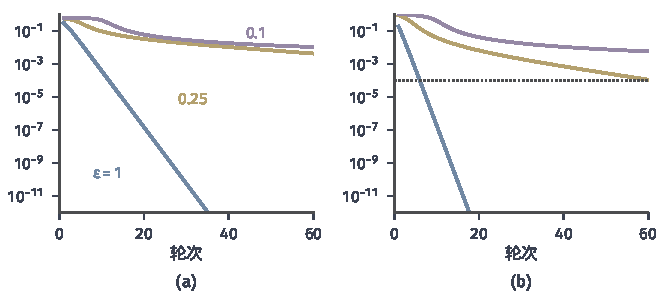
\includegraphics[width=112mm]{figures/07-probability/07-distribution-optimization/matplotlib/ot-sinkhorn-convergence/figure.pdf}
 \caption{全章例子上对数域Sinkhorn迭代的收敛，纵轴为对数刻度：$\varepsilon=1$（蓝）、$0.25$（黄）、$0.1$（紫）。(a)行残差$\rho^{(t)}$。(b)修正后可行方案的原对偶差$\Delta^{(t)}$，深灰点线为容差$10^{-4}$。}
 \label{fig:ot-sinkhorn-convergence}
\end{BookInlineFigure}

\paragraph{三种误差}
用熵正则化近似一个分布之间的运输问题时，最终结果与真正的$\operatorname{OT}_c(\mu,\nu)$之间有三种误差，应分别记录。离散化误差来自把$\mu,\nu$换成有限网格或有限样本上的分布，它取决于网格尺度或样本数。正则化偏差由式~\eqref{eq:ot-entropic-bias}控制，随$\varepsilon$线性减小。迭代误差由停止判据式~\eqref{eq:ot-sinkhorn-stop}控制。减小$\varepsilon$能降低偏差，却使迭代变慢、对数域计算变得必要；三者要在同一预算下权衡，不能只报告其中一项。若最终需要的是原问题的运输成本，还要报告$\langle\bm{C},\tilde{\bm{\pi}}\rangle$而不是正则化目标值。
